\begin{tcolorbox}[colback=red!5,colframe=DarkRed!40!black,title=Entry\, Descent and Landing (EDL)]
Because of Curiosity’s large weight and size, it could not utilize landing procedures used for earlier rovers.
The new landing method is as unique as it is complicated.
The EDL-phase is therefore a spectacle popularly known as \textit{seven minutes of terror} (referring to the time it takes after touching the atmosphere until it lands) \cite{CNN_7minterror}. 

The EDL sequence breaks down into four parts: guided entry, parachute descent, powered descent and the sky crane \cite{NASALanding}. \vspace{2mm}

\begin{center}
	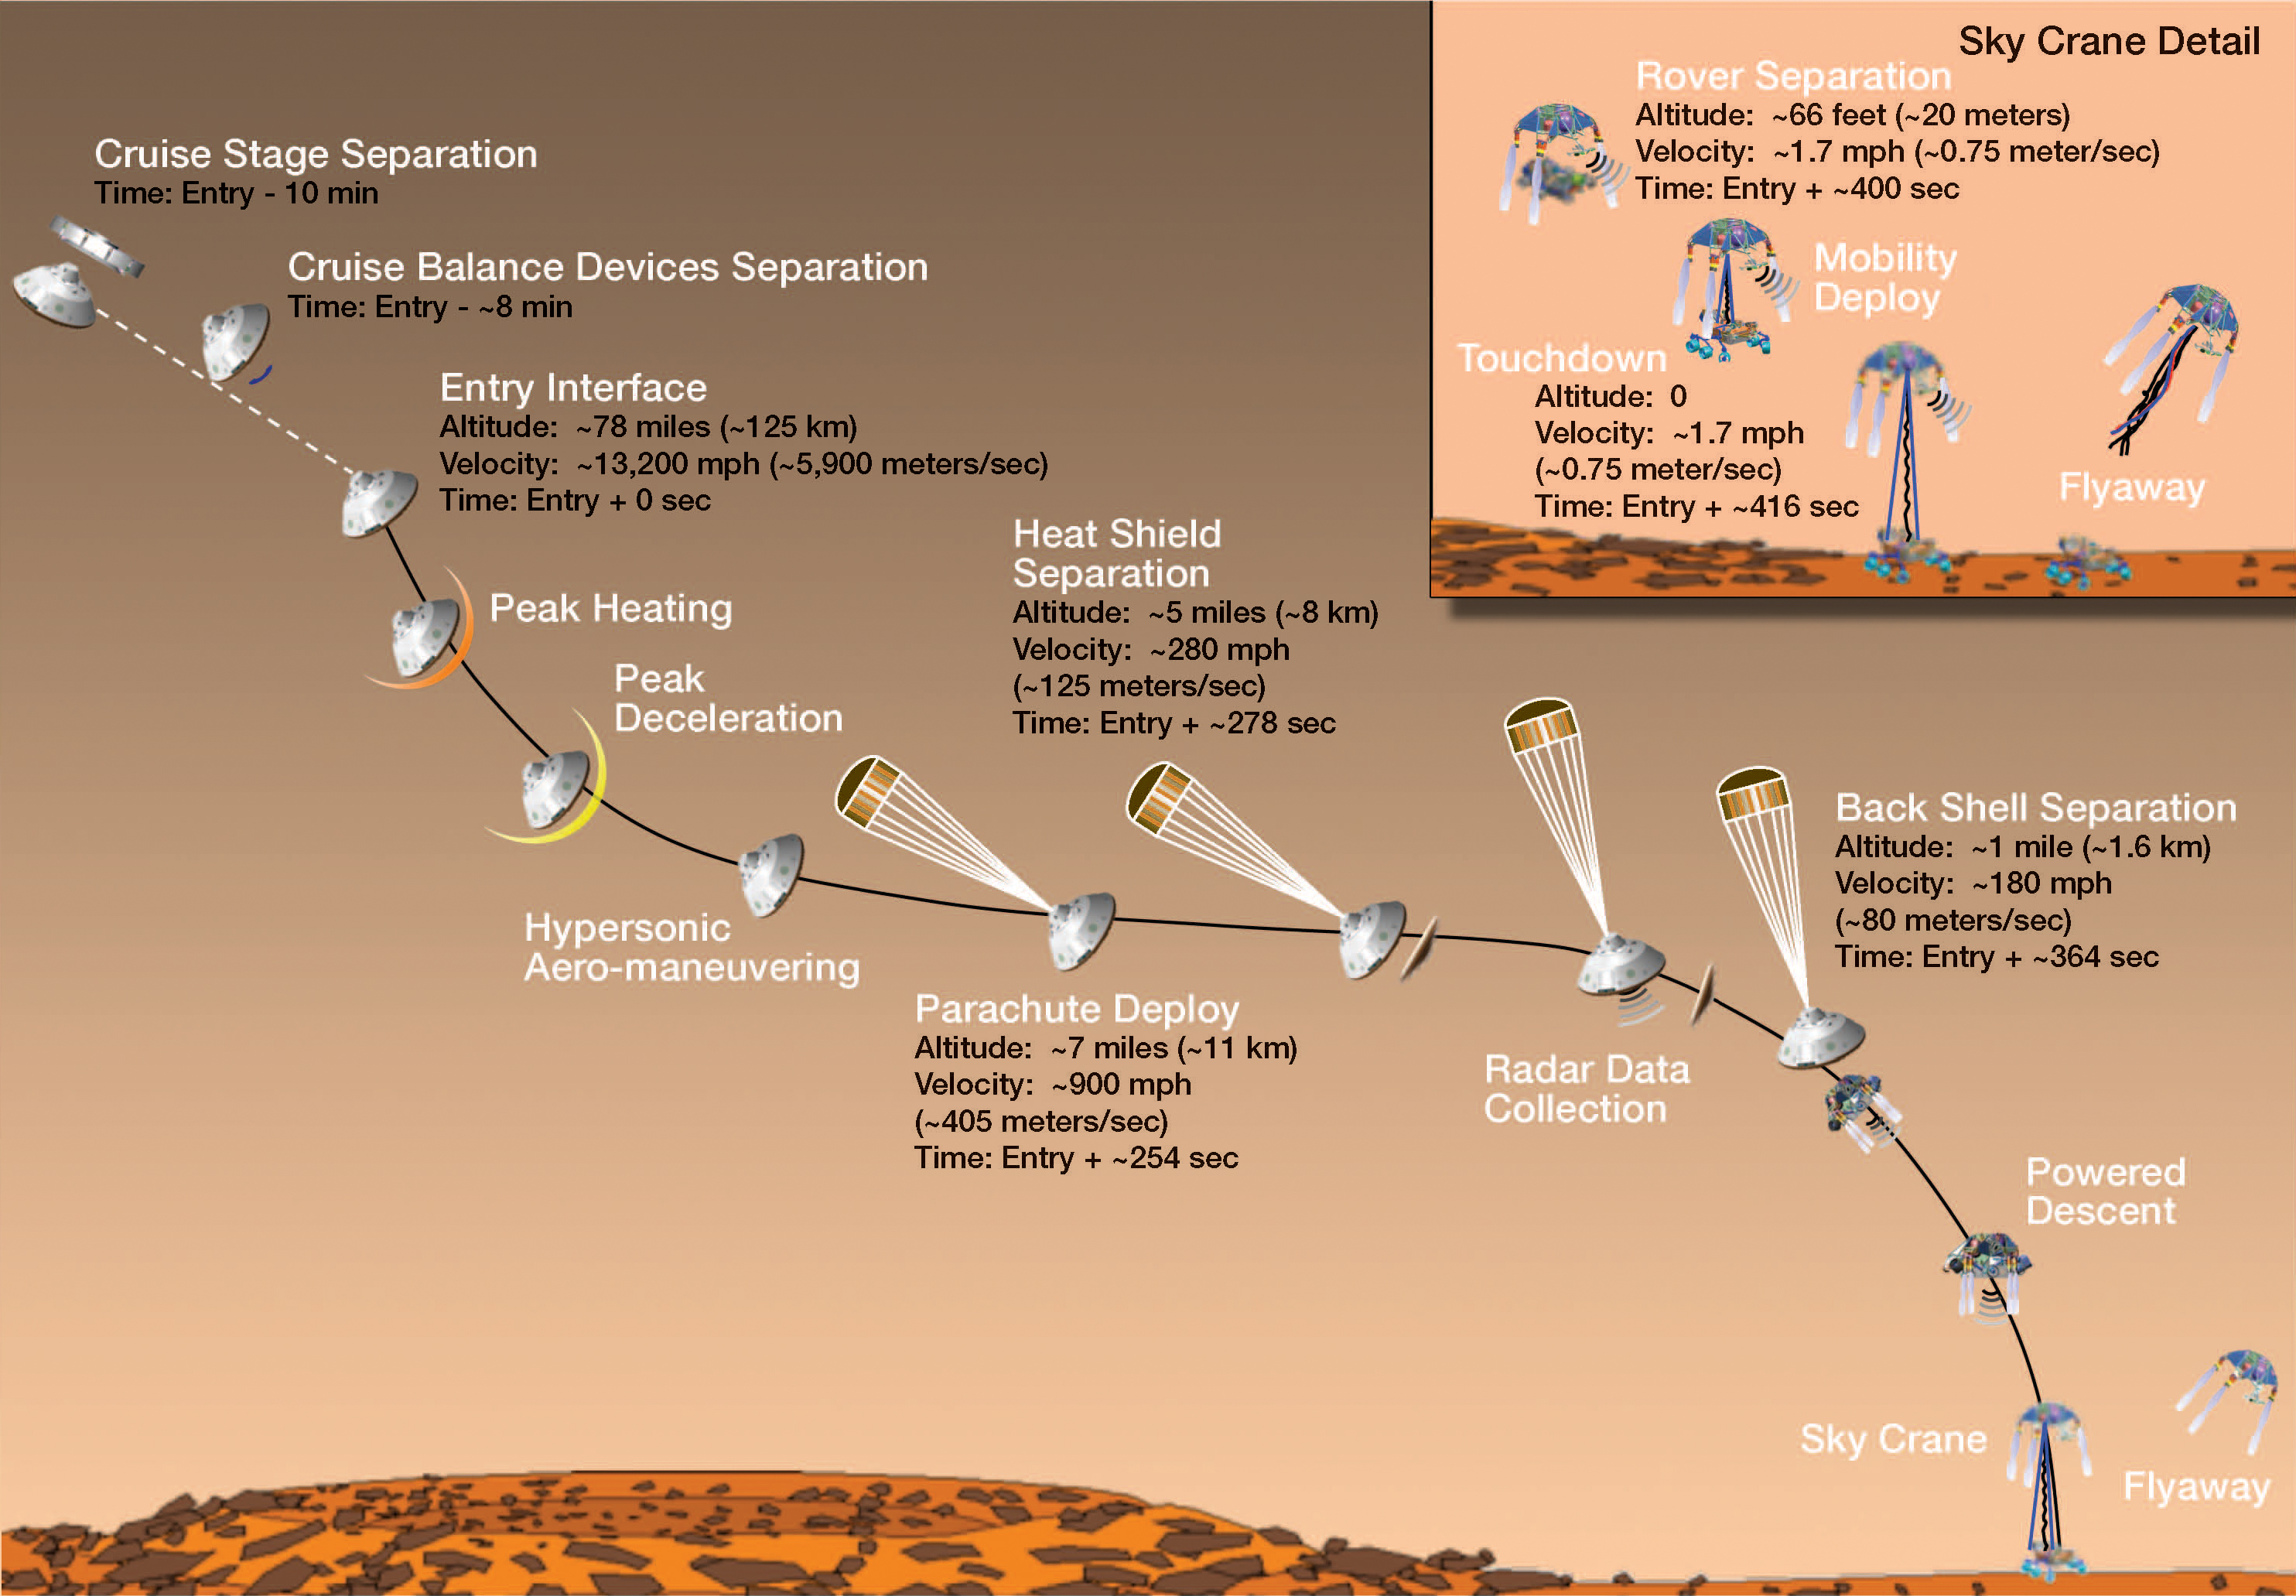
\includegraphics[width=0.9\textwidth]{Curiosity_landing.jpg}
\end{center}

\textbf{Guided entry:}
The spacecraft blasts into the Martian atmosphere at a whopping $21,240 km/h$ creating so much aerodynamic drag the heat shield glows at $2,100 \degree C$ \cite{NASA_youtube}.
The heat shield only manages to slow the spacecraft to a speed of $1,620 km/h$ (because of the thin atmosphere) in which time the deceleration has created a maximum force equal to $16 G$s \cite{HistoricLanding} \cite{NASALanding}.

\textbf{Parachute descent:}
At this point, the largest and strongest supersonic parachute ever constructed for an extra-terrestrial flight deploys.
Capable of generating $24,500 kg$ of drag force the spacecraft decelerates violently to a speed of $280 km/h$ \cite{Parachute} \cite{NASALanding}.
Still way too fast for a landing, there is only one solution: cut the rover loose.

\textbf{Powered descent:}
The rover, now in free fall, accelerates towards the surface at a rate of $3.7 m/s^{2}$, fires eight rocket thrusters and reduces the speed to $14.5 km/h$ while aiming for the landing site \cite{HistoricLanding} \cite{NASALanding}. 

\textbf{Sky Crane:}
At an altitude of $27 m$, the rover is detached from the descent stage and slowly lowered to the ground.
The descent speed is reduced to $2.7 km/h$ and kept constant.
Then finally, on August 6th 2012, after a $5.6 million km$ \cite{CNNCuriosity} journey the rover touches down and pyrotechnically detaches itself from the descent stage.
The decent stage performs a flyaway-maneuver crash-landing $150 m$ away \cite{HistoricLanding} \cite{NASALanding}. Seven minutes of terror completed.
\end{tcolorbox}